\documentclass[../main.tex]{subfiles}
\usepackage[english]{babel}
\graphicspath{{\subfix{../images}}}
\begin{document}


We can think about Neural Networks (NNs) as computational systems inspired by the biological networks of neurons inside the human brain. 
In practical terms, NNs are algorithms able to solve non-linear problems thanks to their complex structure.
The NNs are composed by a high number of connected nodes which are able to learn collectively from the inputs to solve complex tasks \cite{o2015introduction-cnn}.
NNs hide their huge processing power in the links between their elementary units.
The bond strength is  specified by a set of weights, which are tuned by the learning process \cite{gurney2018neural-networks}.

The whole NNs structure might have different architectures, where several neurons layers are organized and connected.
Such layers are composed by single, elementary units called artificial neurons.
To understand how the artificial neural networks are able to learn from simple data and to appreciate how several neurons, bounded into a network, can solve complex problems, it is fundamental to understand the basic functioning of the single neurons.

Inspired by the McCulloch and Pitts studies \cite{mcculloch1943logical-neural-network}, the first artificial neuron was proposed in the late 1950s by Rosenblatt \cite{rosenblatt1958perceptron}.
As shown in Figure \ref{fig:perceptron}, it takes a vector of inputs $x_i$ producing a binary output.

\begin{figure}[H] 
\begin{center}
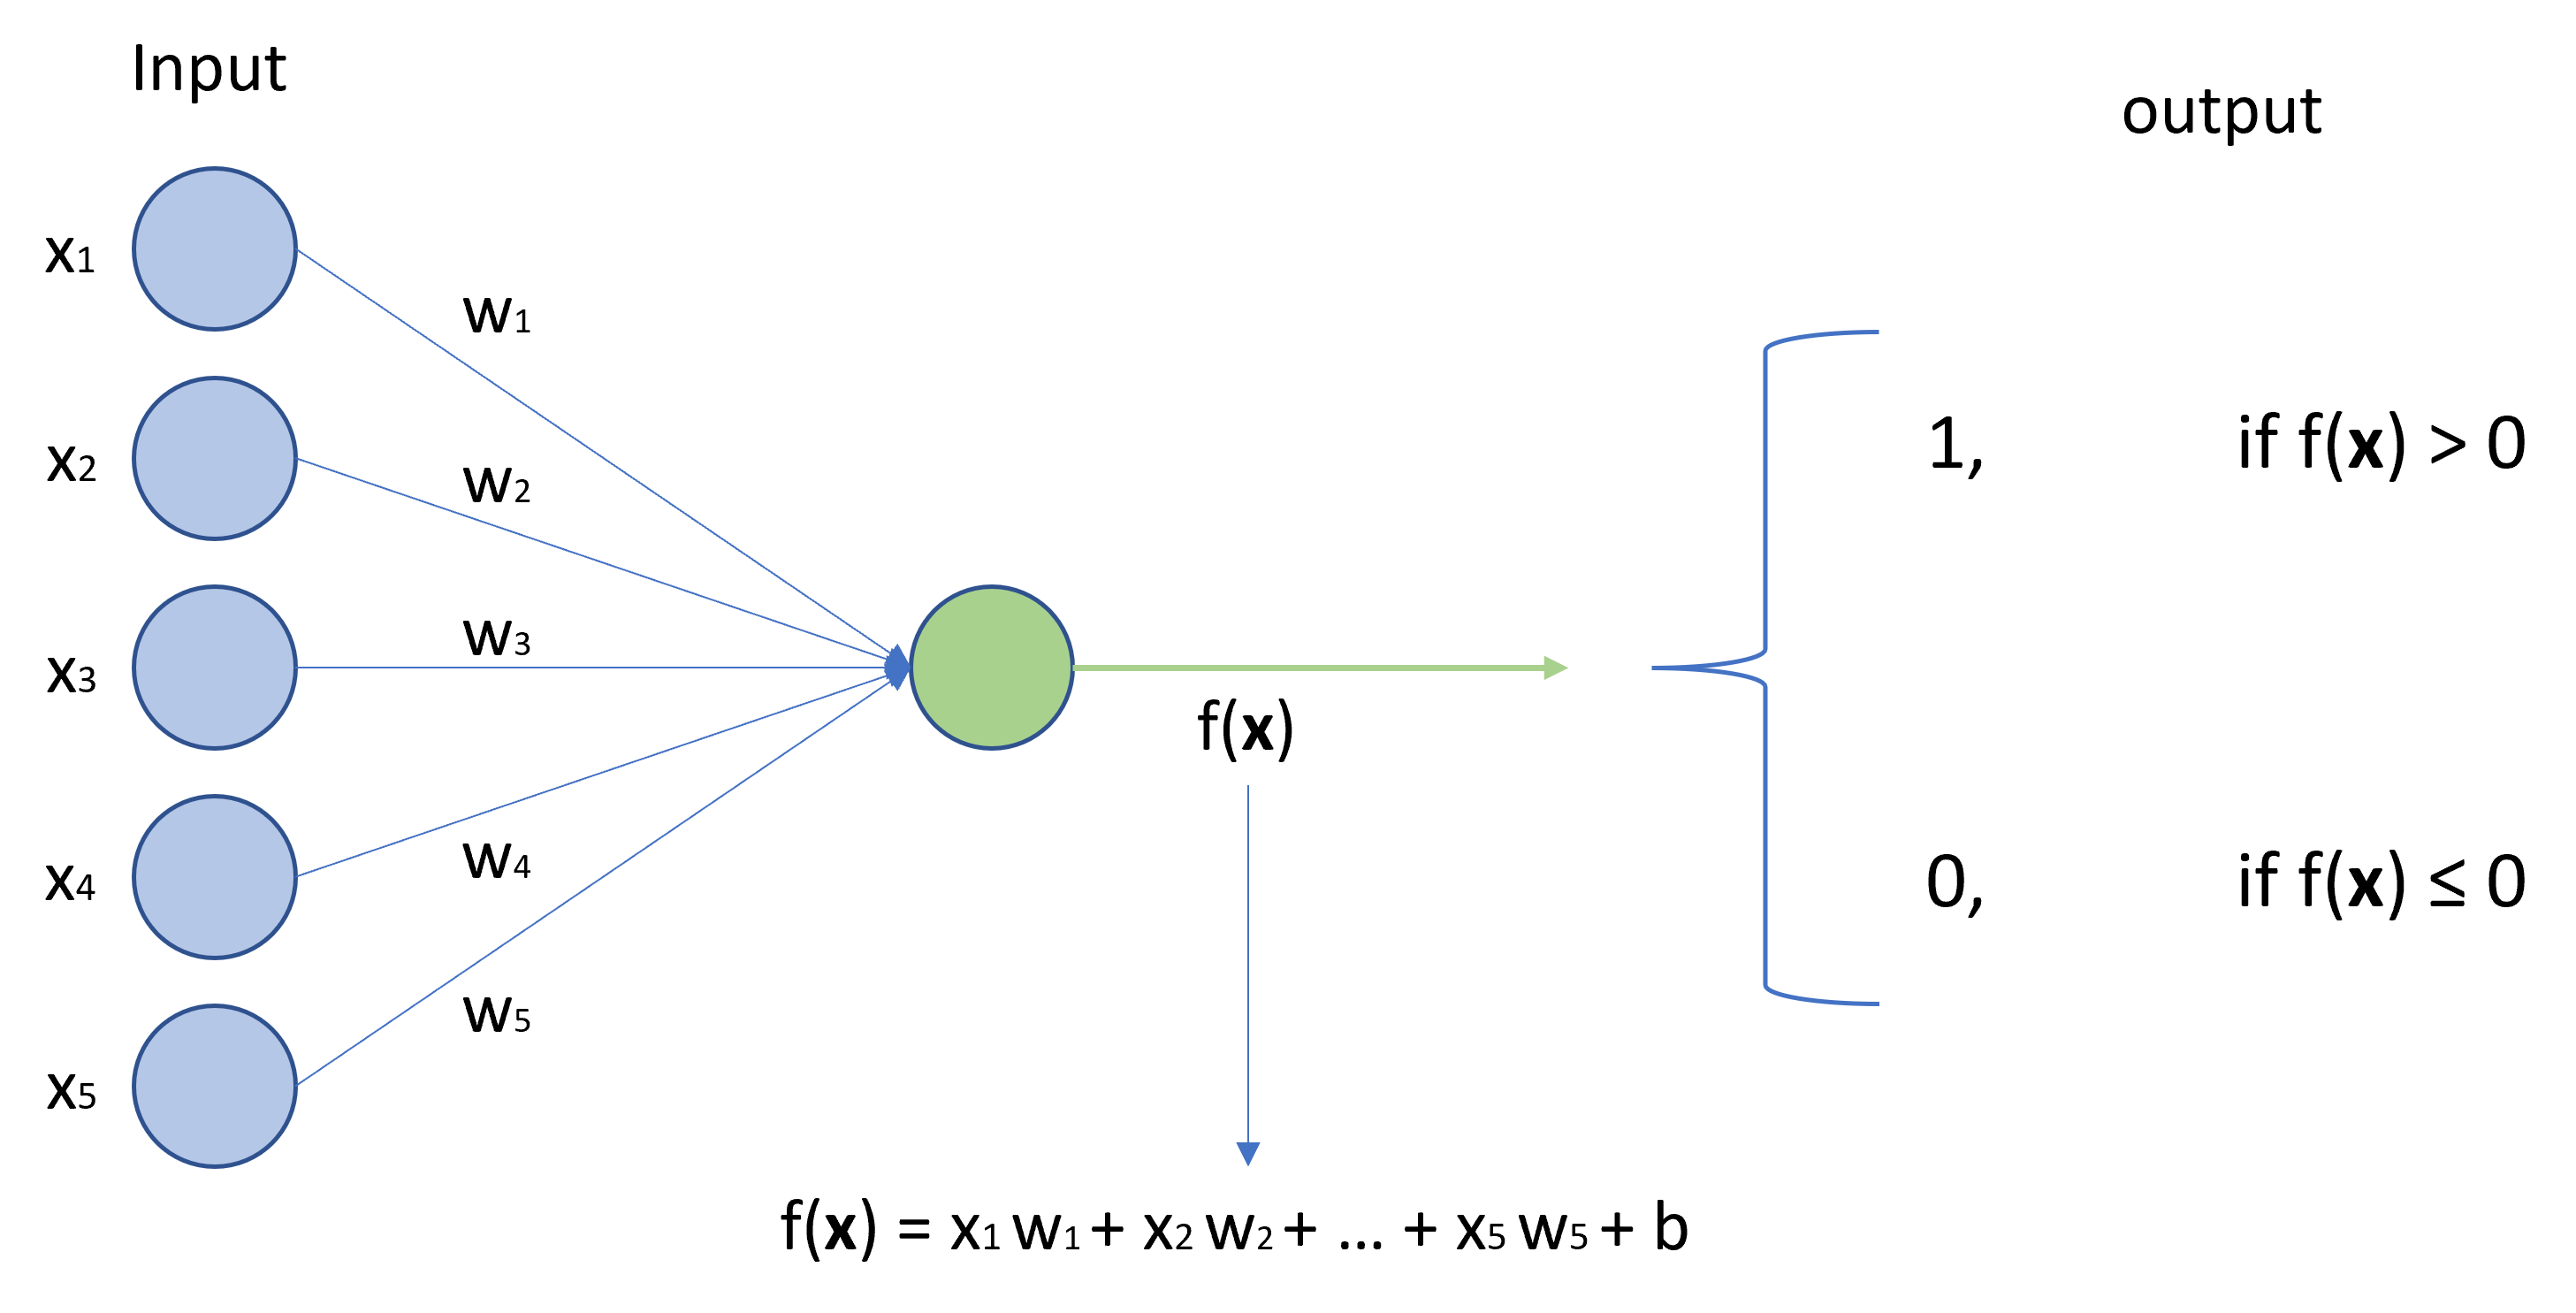
\includegraphics[width=11cm]{images/Perceptron.png}
\caption{\small{Representation of a simple neuron (green circle). The $x_i$ elements are the inputs (blue circles) and the output is calculated based on the weighted sum of these inputs summed with a bias \textit{b}.}}\label{fig:perceptron}
\end{center}
\end{figure}
In the Rosenblatt configuration, the weighted sum of inputs $x_i$ multiplied by the neuron parameters called weights $w_i$ is added to a bias \textit{b}. 
The neuron output is a binary number which depends on the sign of the sum. 
The weights and the bias, which could assume positive or negative values, are the trainable parameters of the model.
They are iteratively changed during the training procedure: if we know what the output for a defined set of inputs $x_{1} \dots x_k$ should be, we can define a cost/error function to estimate the distance from the model result to the known one. 
In this way the model can update its parameters in order to reach an optimal value of the cost function.

As simple as it could appear, the first artificial neuron resembles the functioning of the modern ones with few changes: in modern models numerous  error functions exist and they are chosen according to the task to be solved; moreover, the output of a single neuron is calculated with different \textit{activation functions} which take the previous sum as parameter.

In the following section, Convolutional Neural Networks (CNNs) are explained: they are a peculiar type of NNs universally used to solve image segmentation/classification problems.


\section{Convolutional Neural Networks}

CNNs date back to the 1980s when Fukushima proposed in \cite{fukushima1982neocognitron} the Neocognitron. 
This artificial neuron is inspired by the cat's visual cortex where specific cells, responsive to portion of the total visual field, are stimulated by specific patterns, shapes or orientations \cite{hubel1959receptive-cats}. 

CNNs emulate this biological system by taking a tensor of data instead of a vector, which is particularly useful if we think about the matrix definition of an image in the Equation \ref{eq:image_matrix}.
In this way CNNs are able to exploit correlation between nearby pixels. 
Moreover, the usage of several filters allow CNNs to capture low level feature, as vertical or horizontal edges or colors, in the first layers; proceeding to deeper layers the features extracted are a higher level combination of the previous ones \cite{CNN_chapter13}.
Thus CNNs are able to encode complex image features, which are a key point in images segmentation.

These functions are implemented in the core structure of CNNs with the definition of \textit{convolutional layers}, which are represented in Figure \ref{fig:cnn}.

\begin{figure}[H] 
\begin{center}
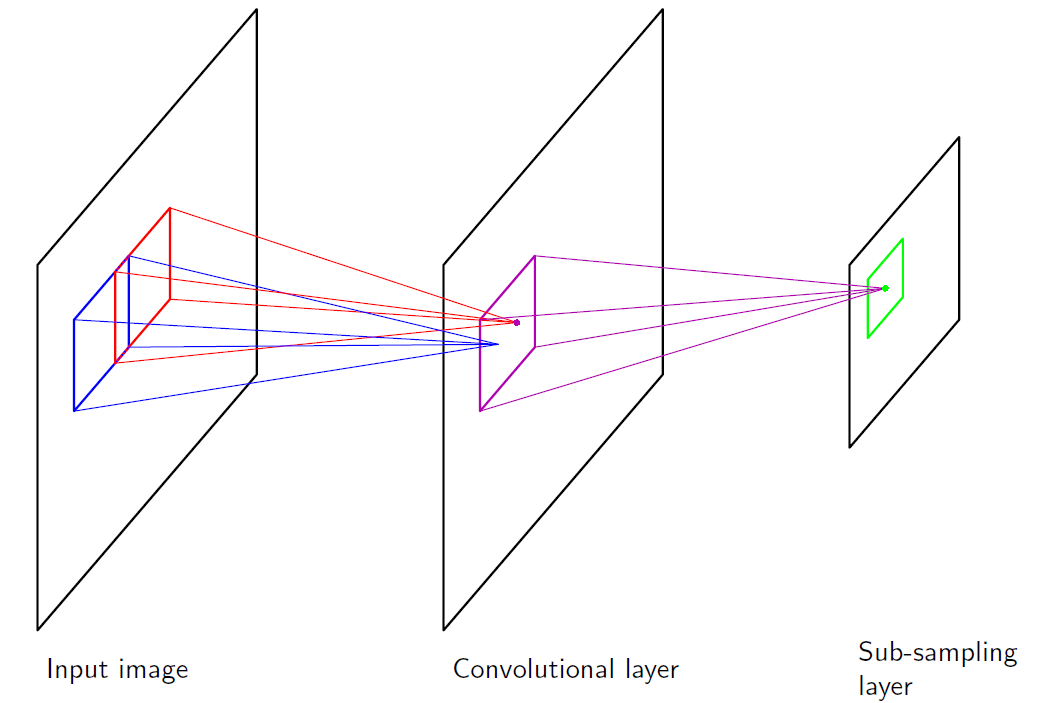
\includegraphics[width=11cm]{images/cnn-layer.png}
\caption{\small{Representation of a portion of a  CNN from \cite{bishop2006pattern}. Portions of the input image (blue and red squares) are mapped into the convolutional layer, then high level features are extrapolated by sub-sampling the result into a successive layer. }}\label{fig:cnn}
\end{center}
\end{figure}
The basic mechanisms of CNNs, responsible for the properties described above, are defined by Bishop in \cite{bishop2006pattern}:

\begin{itemize}
    \item local receptive fields;
    \item parameter sharing;
    \item sub-sampling.
\end{itemize}

Convolutional layers are composed by several planes called \textit{feature/activation maps}, each of those is calculated by a linear combination of parameters with a local region of the input image.
Basically, the single feature map detects a particular pattern at different locations in the image, achieving the aim for local receptive fields.
The parameter sharing is set based on the consideration that patterns are likely to appear in different regions of the same image \cite{o2015introduction-cnn}, thus the same weights are used to calculate the full activation map: having each map characterized by its own set of parameters allow the model to avoid an exponential increase of weights number. 
Lower number of parameters could elude the risk of \textit{over fitting}, a classical behaviour of classifiers with high number of parameters: the model will fit the noise in the data by adapting to peculiar patterns of training set, loosing the ability to generalize with a robust predictive rule \cite{dietterich1995overfitting}.
The sub-sampling stage is a  gradual reduction in spatial dimension of the image, keeping the most informative features calculated in the activation maps without adding more weights to the model.
By stacking several layers together, we appreciate a huge reduction of the spatial dimensions of the image which is compensated by a progressive growth of the feature planes.

Such operations are carried out by two different types of layers: the convolutional one for the accomplishment of local receptive field and the pooling layer for the sub-sampling.

\subsubsection{Convolutional layer}

The fundamental layer in CNNs is the convolutional one. It works by the application of learnable $N\times N$ pixels \textit{kernel} of low spatial dimensions to the full input dimension, by sliding it along the image.
The step size of the sliding path of the kernel is called \textit{stride} and it affects the final output dimension.
The $N\times N$ filter applied  performs a scalar product with a $N\times N$ pixels region of the image.
According to their compositions, kernels are able to highlight specific patterns/orientations inside the image, producing an activation map for each filter applied. 
In some cases techniques of  \textit{zero padding} are used as follows: the borders of the image are enlarged with an array of $0$, in order to end up with greater output dimensions in order to keep borders information in further layers.


A simple formula to calculate the activation map dimension after the convolution layer is presented in \cite{o2015introduction-cnn}, considering a squared $M\times M$ pixels input image the output spatial dimension of the map is:

\begin{equation}
    \frac{(M-N)+2Z}{S+1}
\end{equation}
where $N$ is the kernel dimension, $Z$ is the number of zero padding applied and S is the stride. The \textit{depth} size is the number of feature map produces, which are equal to the number of kernels used in the layer. In this case for a single activation map we will have $N^2 + 1$ trainable parameters, which represent the kernel elements and the bias.

\subsubsection{Pooling layer}

Pooling layer aims to reduce the spatial resolution of the image without increasing the number of parameters of the model. 
It takes activation maps as input and it applies a spatial reduction function. 
The most ones used are average and max function: using a $N\times N$ kernel, such operations are defined, respectively, \textit{average pooling} or \textit{max pooling}.
In both cases a $N\times N$ pixels portion of the activation map is condensed into a single pixel of the pooling layer with the average/max value of the $N^2$ pixels selected, according to the function chosen.
In some case, the pooling operation aims at working with non overlapping regions: to perform a sliding with a $N\times N$ kernel, analysing therefore the used stride is $N$.

A peculiar architecture for CNN is the U-Net network, such name derives from its U-like architecture shape.



\subsection{U-Nets architecture}

The first implementation of the U-Net architecture was proposed by Ronneberger \textit{et al.} in 2015 \cite{ronneberger2015unet}.
It exploits the encoder-decoder structure to perform a pixel-wise classification in the image.
The encoder-decoder power is that it implies the usage of two consequent networks: the first one (encoder) is responsible for the mapping of data into the feature/latent space, producing a multidimensional representation of the image; the second one (decoder) has the aim to reconstruct the original image, taking into consideration the feature extracted for segmentation/classification purposes.
In general, the two networks show the same structure but reversed as shown in Figure \ref{fig:unet}.

\begin{figure}[H] 
\begin{center}
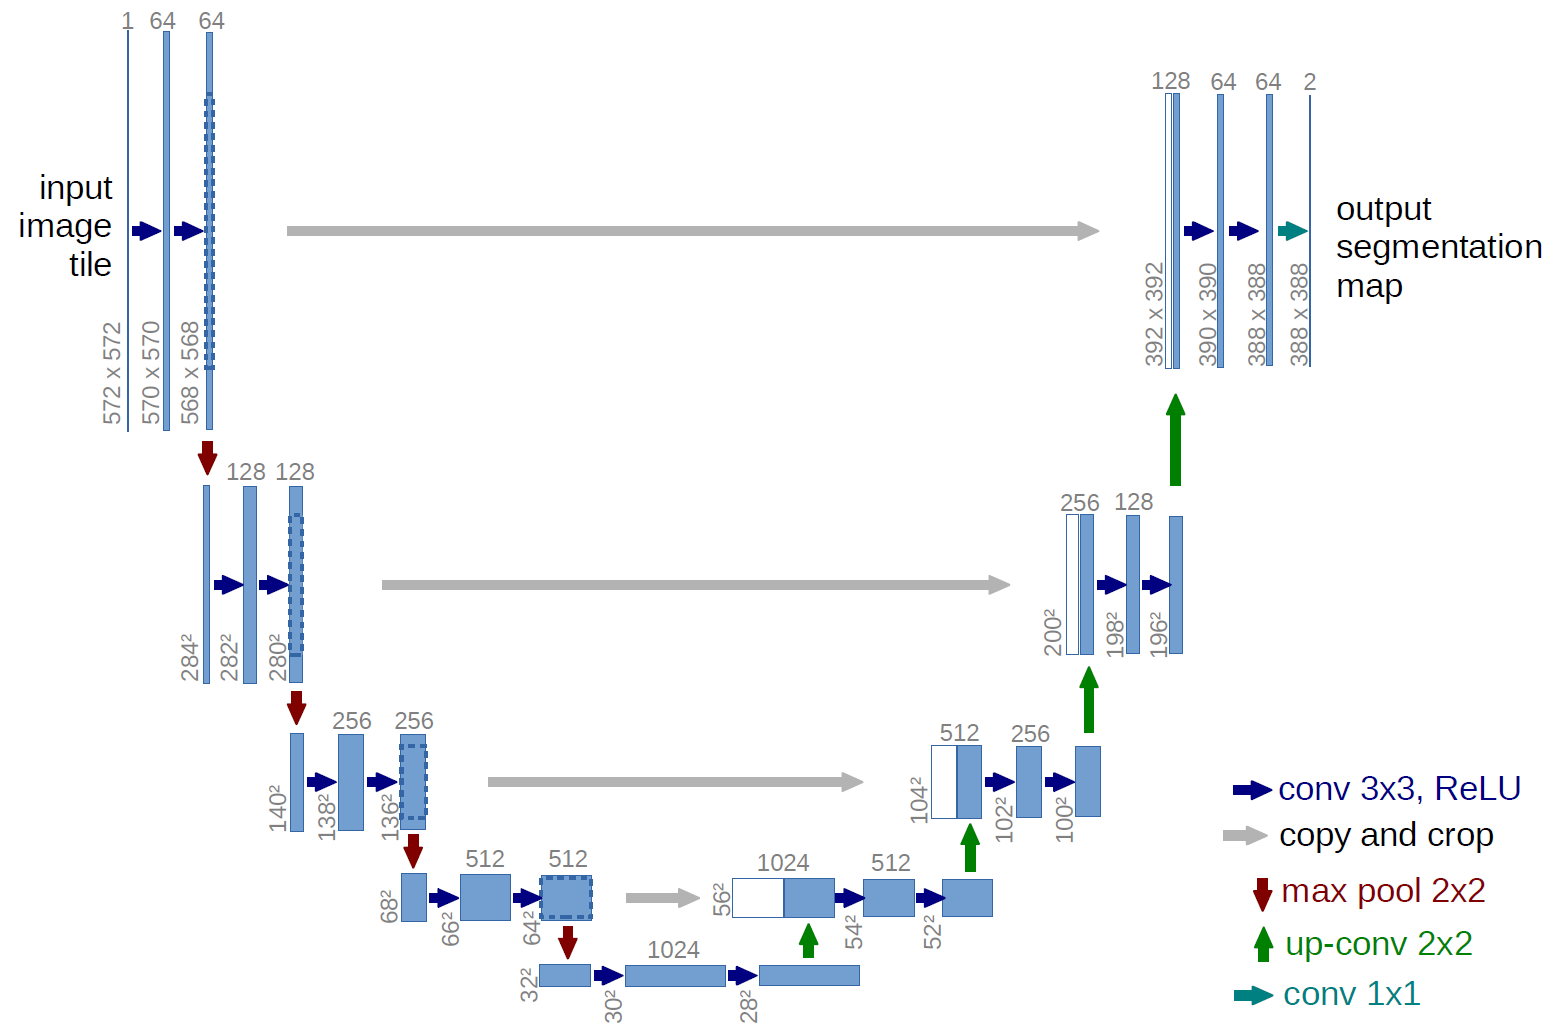
\includegraphics[width=11cm]{images/u-net-architecture.png}
\caption{\small{Architecture of the original U-Net proposed by Ronneberger \textit{et al.} in 2015 \cite{ronneberger2015unet}. Respectively, blue and red arrows represent convolution and sub-sampling;  }}\label{fig:unet}
\end{center}
\end{figure}
The authors proposed a classic network (encoder) as a succession of convolutional layers which transforms the bi-dimensional image input into a multi-dimensional features tensor with low spatial dimensions and high dept; then in the decoder they substituted the pooling operators with up-sampling ones as well as the convolutional ones with up-convolutions.
For each map a ReLu activation function is chosen.
As we can see the output tensor is $N\times N\times 2$ segmentation map in which the information extracted by the U-Net about the foreground and background is contained.
If we would like to perform classification, a deeper output tensor is needed with a depth equal to the number of classes to be detected.

The U-Net architecture represents a family of models which are able to reconstruct the input image, transformed as a segmentation map.
The encoder-decoder structure is divided into two paths.
In the down sampling one (encoder), thanks to several convolutional and pooling layers, a feature tensor is built with high dept. 
This tensor embeds information about the feature vectors of different regions in the image and it is given as input to the decoder.
The decoder path is responsible for the up-sampling phase of the process which combines the features extracted from the encoder.
These features are combined with the up-sampled maps (grey arrows in Figure \ref{fig:unet}) in order to be localized spatially, the successive convolution calculates the output based on both maps. 
The output of the U-Net structure is a 2-depth-dimensional tensor in which the object is separated from the background, thanks to the features coming from the encoder.
The image reconstruction from the tensor representation is calculated by the decoder.


\section{Training the Network}

In ideal situations, network training is performed with many labeled images as reference point for the calculation of the cost function. 
Unfortunately, as already mentioned in \ref{sec:radiomic-pipeline}, manual image segmentation must be executed by experts and it requires a lot of effort and time.
Moreover, labelled datasets able to train a full network, composed by millions of parameters, have to be very large. 

Different learning procedure have been proposed to  overcome the known problem of low/absent labelled data for training.
Before considering such learning solutions, there is a simple solution that focuses on enlarging the quantity of training data to improve performances and to address the problem of over fitting.
These techniques are collected under the name of \textit{Data Augmentation}: such approach tries to address the low labelled data problem by inflating the size of training data with basic image transformations or with the usage of NNs.

\subsection{Data augmentation}

The key idea of data augmentation is that more information can be extracted from the training dataset either warping (manipulation of initial data, preserving labels) or oversampling (creation of synthetic instances).

Following the classification of data augmentation showed in \cite{shorten2019survey-data-augmentation}, the image data augmentation techniques can be sorted in two main categories: image manipulation and deep learning approaches.

\subsubsection{Image manipulation}

Image manipulation consists of a simple transformation of the images, i.e. flipping, rotating, which are able to train the robustness of some invariances of the model. There are many techniques which exploit geometrical or color space properties:

\begin{description}
\item[$\bullet$ Flipping] is the most simple one, collecting both horizontal and vertical flips. In some datasets it could be non label-preserving.
\item[$\bullet$ Cropping] images can be used to reduce image dimensions and it might preserve labels.
\item[$\bullet$ Rotation] could be a useful technique to train rotational invariances.
Some limitations on the angles allowed have to be considered according to the dataset chosen, i.e for recognition of digit numbers we can use only small angles.
\item[$\bullet$ Translating] images is a technique to overcome possible biases due to object position inside the picture.
\item[$\bullet$ Noise injection] is a counter intuitive transformation of the image which adds a random noise value to the pixel matrix in order to learn more robust features.
\item[$\bullet$ Color space transformation] exploits the color channels of the images by considering single colors or by applying transformation of brightness and contrast. It represents a disadvantageous technique if the information heavily depends on the color space.
\item[$\bullet$ Kernel filtering] is the application of filters to the image. It results in images similar to first layers' output of CNNs.
\end{description}

\subsubsection{Deep learning approaches}

Deep learning approaches aim at increasing data by performing alteration in the feature space or by using NNs. The main techniques are:

\begin{description}
\item[$\bullet$ Feature space augmentation] which works by perturbing the data point, exploiting their n-dimensional vector representation in the feature space. 
Such technique is hard to interpret and less effective, compared to image manipulation.
\item[$\bullet$ GAN-based augmentation] refers to the creation of synthetic data with two connected NNs.
The main drawback of this approach is that it needs a lot of training data.
\item[$\bullet$ Neural Style Transfer] is a technique that is able to transfer the style of one image to another, without altering its content. 
Unfortunately, it can introduce new biases inside the training data.
\end{description}
Sometimes data augmentation is not enough to overcome the low labelled data problem. 
In these cases, the selection of particular type of training is needed to train robust NNs.

\subsection{Transfer Learning}\label{sec:tl}

Transfer Learning (TL)  was firstly introduced by Bozinovski in 1976 \cite{bozinovski2020reminder}. It is a learning technique which aims to overcome the absence of labelled data. 
The motivation behind TL is that, in situations where there is no labelled data, it is possible to train a learner from one domain by exploiting transferred information from a similar domain.

The notations to define transfer learning are quite established in different surveys in literature (\cite{weiss2016survey-tranfer-learning1}, \cite{pan2009survey-tranfer-learning2}).

We define a domain $\mathcal{D}$ to be composed by a space $\mathcal{X}$ of features and the probability distribution $P(X)$ with $X=\left\{x_1, \dots, x_n\right\}\in \mathcal{X}$ that represents, for $n$ data points, their feature vectors in the feature space $\mathcal{X}$. 
For a domain $\mathcal{D}=\left\{\mathcal{X}, P(X)\right\}$ we can define the task $\mathcal{T}$ as a label space $\mathcal{Y}$ and a function $f(\cdot)$ which predicts, from the feature vector $x_i \in \mathcal{X}$, the corresponding label $y_i \in \mathcal{Y}$.
From a probabilistic point of view $f(x)$ can be defined as the conditional probability of the label $P(Y|X)$ where $Y=\left\{y_1, \dots, y_n\right\}\in \mathcal{Y}$.

For the TL procedure we define the source domain as $\mathcal{D}_s=\left\{\mathcal{X}_{s}, P(X_{s})\right\}$  with its task $\mathcal{T}_s=\left\{\mathcal{Y}_{s}, f_{s}(\cdot)\right\}$, where $\mathcal{X}_{s}$ is the source feature vector and  $\mathcal{Y}_{s}$ is the source label vector with their respective probabilities; in the same way it is possible to define $\mathcal{D}_t$ and $\mathcal{T}_t$ as target domain and task.

The definition of TL is: given a source domain $\mathcal{D}_s$ with the corresponding source task $\mathcal{T}_s$ and a target domain $\mathcal{D}_t$ with its corresponding target task $\mathcal{T}_t$, TL aims to improve the learning of the target predictive function $f_{t}(\cdot)$ by using the information in $\mathcal{D}_s$ and $\mathcal{T}_s$ for $\mathcal{D}_s\not=\mathcal{D}_t$ or $\mathcal{T}_s\not=\mathcal{T}_t$.

Considering source and target domains $\mathcal{D}_s=\left\{\mathcal{X}_{s}, P(X_{s})\right\}$ and  $\mathcal{D}_t=\left\{\mathcal{X}_{t}, P(X_{t})\right\}$ the inequality $\mathcal{D}_s\not=\mathcal{D}_t$ means that $\mathcal{X}_{s} \not= \mathcal{X}_{t}$ and/or $P(X_{s}) \not= P(X_{t})$ which represent differences in terms of features between domains and/or differences in their marginal distributions, respectively. 
In the same way we can consider source and target tasks with $P(Y|X)$ substituted to $f(\cdot)$, $\mathcal{T}_s=\left\{\mathcal{Y}_{s}, P(Y_{s}|X_{s})\right\}$ and $\mathcal{T}_t=\left\{\mathcal{Y}_{t}, P(Y_{t}|X_{t})\right\}$.
The inequality $\mathcal{T}_s\not=\mathcal{T}_t$ means that  $\mathcal{Y}_{s} \not= \mathcal{Y}_{t}$ and/or $P(Y_{s}|X_{s}) \not= P(Y_{t}|X_{t})$ which represent a difference between label spaces and/or a difference in the conditional probability distributions.

Giving such notation, we can then consider four different cases for learning, according to $\mathcal{D}_s, \mathcal{D}_t$, $\mathcal{T}_s$ and $\mathcal{T}_t$:
\begin{description}
    \item[$\bullet$ $\mathcal{D}_s=\mathcal{D}_t$, $\mathcal{T}_s=\mathcal{T}_t$] : is the trivial case of the classical machine learning methods;
    \item[$\bullet$   $\mathcal{D}_s\not=\mathcal{D}_t$, $\mathcal{T}_s=\mathcal{T}_t$] : is the \textit{Transductive Transfer Learning} where the domains are different but related and the source and target task are the same.
    In this approach labels $Y_{t}$ in the target are not available, but some unlabelled target data $X_{t}$ are given: the learning process aims to adapt the predictive function $f_{s}(\cdot)$ of the source to be used in the target domain through unlabelled data.
    \item[$\bullet$  $\mathcal{D}_s=\mathcal{D}_t$, $\mathcal{T}_s\not=\mathcal{T}_t$] : is the \textit{Inductive Transfer Learning} where  the source and target tasks are different but the domains are the same. 
    The key of this learning procedure is to use part of the labels  $Y_{t}$ in the target domain to induce the predictive function $f_{t}(\cdot)$.  
    \item[$\bullet$  $\mathcal{D}_s\not=\mathcal{D}_t$, $\mathcal{T}_s\not=\mathcal{T}_t$] : is the \textit{Unsupervised Transfer Learning} where source and target tasks are different but related as well as the domains. No labels are available in both source and target domain.
\end{description}

Finally, based on what kind of knowledge we aim to transmit across domains, we can characterize the learning procedure as:

\begin{itemize}
    \item \textit{Instance-transfer} which implies that part of source data can be used successfully for the task in the target domain;
    \item \textit{Feature-representation-transfer} that aims to find a feature representation of the target domain in order to reduce differences between domains;
     \item \textit{Parameter-transfer} that assumes shared parameters between tasks: the transferred knowledge is encoded by the parameters themselves; 
     \item \textit{Relational-knowledge-transfer} which assumes the source and target domains to be similar and the knowledge is shared as relation among data.
\end{itemize}
 
\subsection{Semi-Supervised Learning}

As already mentioned, it could be hard to collect huge amount of labelled data to train you deep learning models. Solutions as Data Augmentation or Transfer Learning may not be enough to overcome the lack of data.

%: increasing training data with augmentation may not be the sufficient for the model to generalize on an independent dataset or related data from witch we can transfer knowledge could not be available.

In such cases it may be useful to exploit Semi-Supervised Learning (SSL) techniques.
Starting from few labelled samples of a dataset, SSL aims to increase the learning performances of the model by adding part of the unlabelled data during the training. Thus the purpose of SSL is to make use of the high number of unlabelled samples to improve model training without increasing workload of human annotators to generate new labelled samples \cite{hady2013semi-supervised}.

We can define SSL adopting the same notation used in TL. 
Recalling the definitions of domain $\mathcal{D}$, task $\mathcal{T}$, feature set $X\in\mathcal{X}$ and label set $Y\in\mathcal{Y}$ of Section \ref{sec:tl}, we can specify a distinction for the SSL framework: we denote $X_{L}$ and $X_{U}$ as the sets of labelled and unlabelled input data, respectively. In general $|X_{L}|<<|X_{U}|$, which means that labelled samples are much less then unlabelled ones.
Thus it is possible to define, for each labelled sample, the couple $\left\{x_{i}, y_{i}\right\}$ of sample and label where $x_{i}\in X_{L}$ and $y_{i}\in Y$, on the other hand for the data points $x_{j}\in X_{U}$ we have no labels. 
We have a successful application of the SSL, for a domain $\mathcal{D}$ and a task $\mathcal{T}$ with two predictive functions $f_{1}(\cdot)$ trained on $X_{L}$ and $f_{2}(\cdot)$ trained on $X_{L}$ and on part of $X_{U}$, when the performances of $f_{2}(\cdot)$ are greater then the performances of $f_{1}(\cdot)$.

SSL methods exploit information embedded in the unlabelled data points to improve the learning ability of the model: this means that a condition for an improvement using SSL is that the data distribution of $P(X)$, where $X = X_{L} + X_{U}$, contains information about the conditional posterior $P(Y|X)$. By including unlabelled data, it is possible to increase knowledge about $P(X)$ and as consequence about $P(Y|X)$.
As pointed out by Van Engelen and Hoos in \cite{van2020survey}, such condition is satisfied in most of the cases; although they suggest that further assumptions have to be stated in order to understand the interaction between $P(X)$ and $P(Y|X)$.

\subsubsection{Smoothness assumption}

For two sample vectors $x_{1}, x_{2} \in \mathcal{X}$ that are close in the feature space, their labels  $y_{1}, y_{2} \in \mathcal{Y}$ should belong to the same class. 
This assumption introduces the concept of proximity, for which even unlabelled data could be assigned to specific classes, if they are close to labelled points.

\subsubsection{Low-density assumption}

This assumption, connected to the previous one, states that the division boundary among classes should pass through low-density regions in the feature space. 
It means that the boundary should be placed in regions where there are few samples.
It is connected to the smoothness assumption since having points which form high density regions implies that their labels are the same, thus no decision boundary could pass through them.

\subsubsection{Manifold assumption}

If we consider the n-dimensional feature space, we could have m-dimensional structures, called \textit{manifolds}, in which points are concentrated, with $m<n$.
The manifold assumption implies the existence of multiple manifolds in the feature space and that points belonging to the same manifold have the same label.
Discovering manifolds could ease the classification of unlabelled data points.\\
\\
It is difficult to evaluate if the application of SSL methods is useful \textit{a priori}. Unlabelled data could improve performances only if they carry information which is not embedded in the labelled ones.
A successful application of SSL is the one which combines SSL with Active Learning (AL), defined as Active Semi-Supervised Learning (ASSL)
\subsubsection{Active Semi-Supervised Learning}

As a branch of SSL, the ASSL aims to make use of unlabelled data, but, instead of using algorithms to label them, queries a human operator. Depending on the task and on the application, ASSL could be very powerful: it may increase the amount of labelled data for the model training successfully with low time.
\end{document}